\chapter{Arquitetura Estabelecida}
\label{chap:Arquitetura}

	Está seção tem como foco detalhar a infraestrutura, isto é, a arquitetura física e lógica estabelecida para desenvolvimento deste projeto. Aqui serão apresentados os componentes da redes e seus especificações técnicas, além de indicar informações de como replicar o ambiente de teste definido.

	\section{Componentes da Arquitetura}
	\label{sec:Arquitetura_Componentes}

		Para montar a infraestrutura necessário para o projeto, utilizou-se de 4 componentes. Cada componente com um papel e serviço específico. Além disso, metade deles são máquina virtuais instânciadas pelo software \emph{VMware}. A seguir, são elencados os componentes e suas respectivas caracteristicas:

		\begin{itemize}
			\item \textbf{Cliente Comum} - IP: \emph{192.168.0.12} - Trata-se da máquina que fará as requisições de aplicações ao servidor principais da rede. Nenhuma ferramenta específica para será utilizada nela, apenas um navegador para as solicitações das requisições.

			\textbf{- Características:} \\
			\textbf{Sistemas Operacional:} Linux Mint 17.2 - 64 bits; \\
			\textbf{Processador:} Intel i5 2.7GHz; \\
			\textbf{Memória RAM:} 2 Gbs; \\
			\textbf{Espaço para Armazenamento:} 80 Gbs; \\
			\textbf{Adaptador de Rede:} Wi-Fi; \\
			\textbf{Ferramentas Instaladas:} Google Chrome V.46.0; \\
			\textbf{É uma máquina virtual?} Sim; \\

			\item \textbf{Cliente Malicioso} - IP: \emph{192.168.0.13} - Trata-se da máquina que fará os ataques a rede. Neste caso, este componente sempre tentará atacar o servidor principal, tentando na maioria das vezes derruba-lo. Para esta máquinas utilizou-se um sistema operacional específico para auditorias e segurança de computadores \cite{kali}. Todas as ferramentas utilizadas para os ataques são nativas ao sistema operacional.

			\textbf{- Características:} \\
			\textbf{Sistemas Operacional:} Kali Linux 2.0 - 64 bits; \\
			\textbf{Processador:} Intel i5 2.4GHz; \\
			\textbf{Memória RAM:} 4 Gbs; \\
			\textbf{Espaço para Armazenamento:} 200 Gbs; \\
			\textbf{Adaptador de Rede:} Wi-Fi; \\
			\textbf{Ferramentas Instaladas:} Ping, NMAP, Zenmap, HPING3, Hydra; \\
			\textbf{É uma máquina virtual?} Não; \\

			\item \textbf{Servidor IPS/IDS} - IP: \emph{192.168.0.42} - Trata-se do servidor que monitora a rede. Neste componente se encontra a ferramenta IPS/IDS devidamente configurada para o monitoramento. Foi utiliado um sistema operacional específico para detecção de intrusões, monitoramento de rede e gerenciamento de log \cite{SO}. Todas as ferramentas utilizadas para os ataques são nativas ao sistema operacional.

			\textbf{- Características:} \\
			\textbf{Sistemas Operacional:} Security Onion 12.04 - 64 bits; \\
			\textbf{Processador:} Intel i3 1.9GHz; \\
			\textbf{Memória RAM:} 4 Gbs; \\
			\textbf{Espaço para Armazenamento:} 150 Gbs; \\
			\textbf{Adaptador de Rede:} Wi-Fi; \\
			\textbf{Ferramentas Instaladas:} Snort e Snorby; \\
			\textbf{É uma máquina virtual?} Não; \\

			\item \textbf{Servidor Principal} - IP: \emph{192.168.0.17} - Trata-se de um servidor com alguns serviços FTP, SSH, TCP entre outros. Também foi utilizado um sistema operacional específico para este componente. Neste caso, a máquina é intencionalmente vulnerável, comumente utilizada para testes de segurança em redes como técnicas de intrusão por exemplo \cite{metasploitable2}.

			\textbf{- Características:} \\
			\textbf{Sistemas Operacional:} Metasploitable2 2.0 - 64 bits; \\
			\textbf{Processador:} Intel i3 1.9GHz; \\
			\textbf{Memória RAM:} 4 Gbs; \\
			\textbf{Espaço para Armazenamento:} 150 Gbs; \\
			\textbf{Adaptador de Rede:} Wi-Fi; \\
			\textbf{Ferramentas Instaladas:} Apache, vsftpd, Open SSH; \\
			\textbf{É uma máquina virtual?} Sim; \\

		\end{itemize}


	\section{Esquema da Infraestrutura}
	\label{sec:Arquitetura_Esquema_Infra}

		A figura \ref{fig:arquitetura} encontra-se a representação lógica da estrutura de redes estabalecida para este projeto.

		\begin{figure}[h]
			\centering
			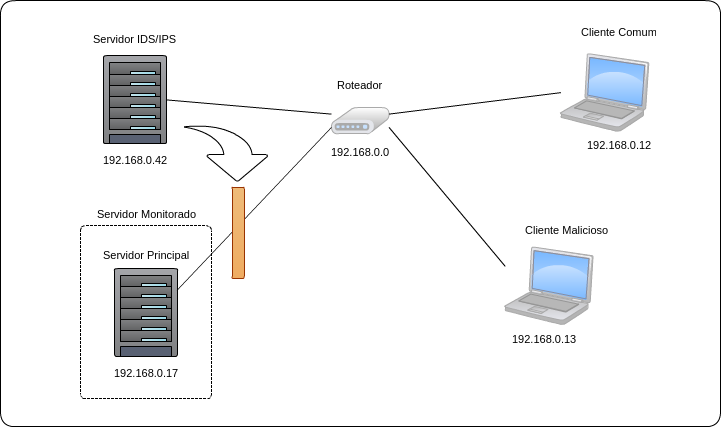
\includegraphics[scale=0.6]{arquitetura}
			\caption{Arquitetura estabelecida para o Projeto.}
			\label{fig:arquitetura}
		\end{figure}

		Percebe a configuração de uma topologia estrela, neste caso, 4 componentes são interligados através de comutador central. Nesta configuração de rede, todas as informações enviada de um nó para outro passa primeiramente pelo elemento central (comutador) antes de chegar a outro nó, portanto, as informações não passam de um host para o outro diretamente. \cite{Tanenbaum}

		Uma das principais vantagens dessa topologia é a administração central, pois ocorrendo algum problema em uma das extremidades, a arquitetura não será totalmente comprometida mas, apenas no host com problema. Em contrapartida, qualquer problema no equipamento central, toda a arquitetura é paralisada.

	\section{Instalação das Ferramentas}
	\label{sec:Arquitetura_Componentes}

		Neste tópico são apresentados os procedimentos para instalação das principais ferramentas utilizadas. Algumas ferramentas utilizadas são nativas de determinados sistemas operacionais, no entanto, apresentam-se pequenos tutoriais de como instalar cada uma das ferramentas. Na primeira subseção são apresentados os sistemas operacionais utilizados e na segunda subção as principais ferramentas.

		Ressalta-se ainda a utilização de um sistema operacional baseado no Unix, assumindo-se o Ubuntu 14.04 como sistema base para as instalações. Além disso, evitou-se ao máximo trazer tutoriais de configurações de ferramentas para este relatório a fim de não sobrecarrega-lo com uma série de comando de configuração, uma vez que algumas dessas ferramentas rapidamente tornou-se obsoletas. No entanto, em todos as ferramentas que forem necessárias configurações específicas, foram apresentados os respectivos \emph{links} utilizados para tais configurações.

		\subsection{Sistemas Operacionais Utilizados}
		\label{sec:Arquitetura_Componentes_SOU}

			Nesta subseção são apresentados os sistemas operacionais utilizados para executar o projeto.

			\begin{itemize}

				\item \textbf{Linux Mint} - Trata-se de uma distro do sistema operacional Linux, baseada nas distros Ubuntu e Debian. O Mint oferece muitas vantagens, uma de suas principais é a simplicidade e elegância visual voltado ao usuário final. \cite{mint}

				Para efetuar o download, instalação e configuração utilizado-se a documentação base do sistema operacional. Disponível em:

				\begin{framed}
					\href{http://www.linuxmint.com/documentation.php}{http://www.linuxmint.com/documentation.php}
				\end{framed}
				\textbf{Fonte:} Official Linux Mint Documentation.


				\item \textbf{Kali Linux} - Trata-se de uma distro específica para auditorias e segurança de computadores. O Kali possui um arsenal de ferramentas que proporcionam diversas invasões, além de inúmeros ataques a redes. \cite{kali}

				Para efetuar o download, instalação e configuração utilizado-se a documentação base do sistema operacional. Disponível em:

				\begin{framed}
					\href{http://docs.kali.org/introduction/}{http://docs.kali.org/introduction/}
				\end{framed}
				\textbf{Fonte:} Official Kali Linux Documentation.

				Adicionalmente, para a instalação de todas as ferramentas necessárias para efetuar os testes, ao final da instalação do sistemas operacional, executou-se o comando a seguir:

				\begin{framed}
					\textbf{sudo apt-get install kali-linux-all}
				\end{framed}


				\item \textbf{Security Onion} - Trata-se de uma distro específica para detecção de intrusões, monitoramento de rede e gerenciamento de log. O Security Onion possui diversas ferramentas estilo forense, destinadas a principalmente a IDS e NSM, sendo uma plataforma muito útil para perícias. \cite{SO}

				Para efetuar o download, instalação e configuração utilizado-se a documentação base do sistema operacional. Disponível em:

				\begin{framed}
					\href{https://security-onion-solutions.github.io/security-onion/}{https://security-onion-solutions.github.io/security-onion/}
				\end{framed}
				\textbf{Fonte:} Official Security Onion Documentation.


				\item \textbf{Metasploitable2} - Trata-se de uma distro baseada no Ubuntu específica para testes de segurança uma vez que ela é intencionalmente vulnerável. Comumente são utilizadas técnicas de intrusão, ataques de DoS entre outros a fim de atestar a efetividade de métodos de proteção. Além disso, em seu site oficial, o Metasploitable2 é oferecido para download como uma máquina virtual, diferentemente dos outros sistemas operacionais anteriormente detalhados \cite{metasploitable2}.

				Para efetuar o download, instalação e configuração da máquina virtual utilizado-se a documentação base do sistema operacional. Disponibilizada pela comunidade em:

				\begin{framed}
					\href{https://community.rapid7.com/docs/DOC-1875}{https://community.rapid7.com/docs/DOC-1875}
				\end{framed}
				\textbf{Fonte:} Official Metasploitable2 Documentation.

			\end{itemize}


		\subsection{Principais Ferramentas Utilizados}
		\label{sec:Arquitetura_Componentes_PFU}

			Nesta subseção são apresentados as principais ferramentas utilizados para executar o projeto.


			\begin{itemize}

				\item \textbf{Ping} - Trata-se do comando de teste para conectividade entre equipamento. É comumente nativo aos sistemas operacionais baseados no Unix.

				A demostração da utilização desta ferramenta é abordada no capitulo \ref{chap:Simulacao} - \nameref{chap:Simulacao} - Tópico \ref{sec:Geracao_de_Ruido_com_Ping} - \nameref{sec:Geracao_de_Ruido_com_Ping}.


				\item \textbf{NMAP} - Trata-se de uma ferramenta para exploração de portas, isto é, scanner de portas. \cite{nmap}

				Para efetuar a instalação, digita-se:
				\begin{framed}
					\textbf{sudo apt-get install nmap}
				\end{framed}

				A demostração da utilização desta ferramenta é abordada no capitulo \ref{chap:Simulacao} - \nameref{chap:Simulacao} - Tópico \ref{sec:Geracao_de_Ruido_com_FootPrint} - \nameref{sec:Geracao_de_Ruido_com_FootPrint}.


				\item \textbf{Zenmap} - Trata-se de uma ferramenta que visa facilitar a utilização do NMAP para iniciantes e fornecer recursos mais avançado a usuários mais experiêntes. \cite{zenmap}

				Para efetuar a instalação, digita-se:
				\begin{framed}
					\textbf{sudo apt-get install zenmap}
				\end{framed}

				A demostração da utilização desta ferramenta é abordada no capitulo \ref{chap:Simulacao} - \nameref{chap:Simulacao} - Tópico \ref{sec:Geracao_de_Ruido_com_FootPrint} - \nameref{sec:Geracao_de_Ruido_com_FootPrint}.


				\item \textbf{HPING3} - Trata-se de uma ferramenta que encaminha pacotes TCP/IP personalizados. Para este projeto, a ferramenta foi utilizada para encaminhar vários pacotes SYN Flood.

				Para efetuar a instalação, digita-se:
				\begin{framed}
					\textbf{sudo apt-get -y --force-yes install hping3}
				\end{framed}

				O comando \emph{--force-yes} forçará a opção "yes" em todas as telas apresentadas durante a instalação.

				A demostração da utilização desta ferramenta é abordada no capitulo \ref{chap:Simulacao} - \nameref{chap:Simulacao} - Tópico \ref{sec:Flood_Attack} - \nameref{sec:Flood_Attack}.


				\item \textbf{Hydra} - Trata-se de uma ferramenta clássica usada para quebrar senhas. Ele utilizado a técnica de força bruta para quebrar senhas.

				Para efetuar a instalação, digita-se:
				\begin{framed}
					\textbf{sudo apt-get install hydra}
				\end{framed}

				A demostração da utilização desta ferramenta é abordada no capitulo \ref{chap:Simulacao} - \nameref{chap:Simulacao} - Tópico \ref{sec:Brute_Force_SSH} - \nameref{sec:Brute_Force_SSH}.


				\item \textbf{Snort} - Trata-se de uma ferramenta de detecção de intrusão na rede(NIDS) flexível em suas configurações de regras.

				Para utilização da ferramenta é necessário a instalação do MySQL, um dos bancos de dados mais populares. Para tanto, digita-se o comando:
				\begin{framed}
					\textbf{sudo apt-get install snort-mysql}
				\end{framed}

				Para efetuar a configuração da ferramenta, utilizou-se o tutorial apresentado no link a seguir:

				\begin{framed}
					\href{http://www.vivaolinux.com.br/artigo/Snort-MySQL-Guardian-Instalacao-e-configuracao?pagina=2}{http://www.vivaolinux.com.br/artigo/Snort-MySQL-Guardian-Instalacao-e-configuracao\?pagina=2}
				\end{framed}
				\textbf{Fonte:} Viva o Linux.

				A demostração da utilização desta ferramenta é abordada durante o desenvolvimento do capitulo \ref{chap:Simulacao} - \nameref{chap:Simulacao}.


				\item \textbf{Snorby} - Trata-se de uma ferramenta de frontends utilizados para visualizar os alertas gerados pela ferramenta Snort citada anteriormente.

				Para utilização da ferramenta é necessário a instalação do MySQL além de outras ferramentas requisitos para o Snorny. Portanto, para efetuar a instalação e configuração, utilizou-se o tutorial apresentado no link a seguir:

				\begin{framed}
					\href{http://www.vivaolinux.com.br/artigo/SAMSB-Snort-+-Apache2-+-MySQL-+-Snorby-e-BarnYard2-no-Debian?pagina=2}{http://www.vivaolinux.com.br/artigo/SAMSB-Snort-+-Apache2-+-MySQL-+-Snorby-e-BarnYard2-no-Debian\?pagina=2}
				\end{framed}

				\textbf{Fonte:} Viva o Linux.

				A demostração da utilização desta ferramenta é abordada durante o desenvolvimento do capitulo \ref{chap:Simulacao} - \nameref{chap:Simulacao}.

			\end{itemize}

	\section{Limitações e Dificuldades}
	\label{sec:Arquitetura_Limitacoes}

		\subsection{Intalação das Ferramentas}
			Para o desenvolvimento do trabalho de implementação do sistema IDS/IPS é
			necessário instalar uma sequência de ferramentas que possibilitam a implantação
			do sistema bem como o teste do mesmo. As principais ferramentas utilizadas
			neste trabalho foram: Snort e Snorby. Ambas, apesar de muito comuns no mercado,
			tem um processo de configuração muito particular do ambiente de utilização
			da mesma. O grupo encontrou muitas dificuldades para configurar no ambiente
			de teste, pois, a dinâmica de padronização era desconhecida.

		\subsection{Configuração das Ferramentas}
			Estabelecer uma interface para a captura de pacotes também foi um implecílio
			encontrado, pois o processo de configuração era manual e não se compreedia
			como deveria ser procedido. Para a resolução do problema, foi utilizado o
			sistema operacional Security Onion, que já possui todas as ferramentas
			utilizadas no nosso trabalho com relação à segurança.

		\subsection{Restrições Físicas}
			Após configuradas as interfaces, observou-se que o Snort estava capturando
			apenas os pacotes que utilizam a rede eth0 para trafegar. Porém, a rede de
			simulação estava instalada longe do roteador, logo, todas as máquinas estavam
			conectadas via wifi. Assim, fez-se necessário por parte do proprietário das
			máquinas adquirir vinte metros de cabo ethernet a fim de interligar os
			computadores pela inteface eth0.

		\subsection{Execução dos Ataques}
			A execução dos ataques foi um ponto complexo, pois, apesar se simples, exige
			uma quantidade de conhecimento considerável para entender o processo que
			estava sendo execudado no backend, a fim de testar as regras no sistema
			de detecção e prevenção de intrusos.

			Para testar as regras, era necessário conhecer sobre os dados trafegantes
			ao identificar as recorrências.
